\chapter{Viewing volumetric data}\label{ch:volume}
\index{Volumetric data}

\chapterlead{An atomic structure tells you where the atoms are; volumetric data describes how numerical values vary throughout space. Charge density, magnetization density, and other scalar fields can be viewed as isosurfaces, slices, or direct volume renderings. Using CHGCAR, Cube, and XSF examples, this chapter explains how to select channels, interpret units, compare views, and export figures and data for reports or further analysis.}

\section{Understand the data}
\index{Charge density}
\index{Volumetric data!Channels}

\subsection{What a volumetric dataset represents}

A three-dimensional scalar field is a set of values on a spatial grid. Each grid point has a position and a scalar value; the viewer interpolates between neighboring points to produce a continuous display. The grid dimensions specify the number of samples in each direction. The voxel vectors, origin, and cell determine their positions in real space.

A grid need not be orthogonal or aligned with the Cartesian axes. In a skewed cell or a dataset from another program, slices may therefore be tilted. Check the file's source, dimensions, and units before relating the field to the atomic structure.

One file can contain several channels. For example, a spin-polarized CHGCAR contains both total charge density and magnetization information, and a Cube file can contain multiple datasets. Changing the channel changes the scalar field being displayed, rather than merely its colors.

\begin{table}[htbp]
\centering
\caption{Common volumetric formats and their interpretation in the viewer.}
\begin{tabularx}{\linewidth}{lX}
\toprule
File & Contents and interpretation \\
\midrule
CHGCAR, CHG & VASP scalar grids and atomic structures. Charge density is normalized by the cell volume and displayed in $\text{\AA}^{-3}$; spin-polarized files provide additional channels.\\
Cube, CUB & An origin, voxel vectors, atoms, and one or more datasets. The scalar's physical meaning depends on the program and calculation that produced it.\\
XSF & Labeled two- or three-dimensional datagrids, optionally with atomic structures. Identify each grid block and channel by its label.\\
\bottomrule
\end{tabularx}
\end{table}

Cube and XSF values are not universally interpreted as electron density; the interface may show \file{arbitrary} as the unit. This means that the viewer retains the source values without assigning the same physical unit to every file. Even if a field resembles a charge distribution, interpret its values according to the calculation that produced it.

\subsection{Spin channels in \headinglatin{CHGCAR}}
\index{CHGCAR}

A non-spin-polarized CHGCAR normally uses \file{total}. For collinear spin data, \file{diff} is the magnetization density associated with the spin difference. The viewer also provides derived \file{up} and \file{down} channels:
\[
  \rho_{\uparrow}=\frac{\rho_{\mathrm{total}}+\rho_{\mathrm{diff}}}{2},
  \qquad
  \rho_{\downarrow}=\frac{\rho_{\mathrm{total}}-\rho_{\mathrm{diff}}}{2}.
\]
Negative \file{diff} values indicate the sign of the spin difference, not a negative total electron density. Noncollinear data can also contain the three magnetization components and their magnitude. Distinguish signed components from a vector magnitude when interpreting them.

\section{Import volumetric data}

\begin{steps}
  \item Open the \ui{Project Browser} from the sidebar, double-click the top-level \ui{Volume} category, and select a volumetric file. Start with \file{CHGCAR.nospin.gz}. If the project tree is hidden, select \ui{Project Browser} from the sidebar's \ui{Open Panels} gallery.
  \item Wait for the initial view and summary. Check the filename, \ui{Grid} dimensions, and \ui{Units} to confirm that the intended dataset is open.
  \item Drag with the left mouse button to rotate, scroll to zoom, and drag with the right button to pan. Press Space to center the view and fit the model.
  \item Open \ui{Viewer settings} on the volume view's own toolbar and inspect \ui{Channel} and \ui{Display mode}. Identify the channel and mode before changing the appearance.
  \item If the file includes an atomic structure, retain the cell and atom overlays to see where the field lies relative to the atoms.
\end{steps}

A large dataset may initially appear at reduced display resolution before the full data loads. The status area can report loading, construction, or a fallback mode. Wait for completion before recording the grid or preparing a final figure, so that an initial preview is not mistaken for the complete dataset.

The toolbar also provides automatic rotation, lattice- and reciprocal-axis views, structure information, image export, scene-description export, and full screen. Press I to hide or restore supporting elements such as the summary and distribution plot. Restore them when recording values and units.

Imported volumes appear below \ui{Volume}; double-click a specific item to reopen it. The top-level category imports a new file, while child items open existing data. Sidebar panels manage the project; settings inside the volume view control the image. Use the latter for atom scale, channels, and slices.

Figure~\ref{fig:volume-total-isosurface} shows the total charge density from the supplied non-spin-polarized file. The pale blue isosurface is displayed with the cell and atoms, making its position relative to the structure easier to judge. The next section explains how to check the file, channel, and threshold.

\begin{figure}[H]
\centering
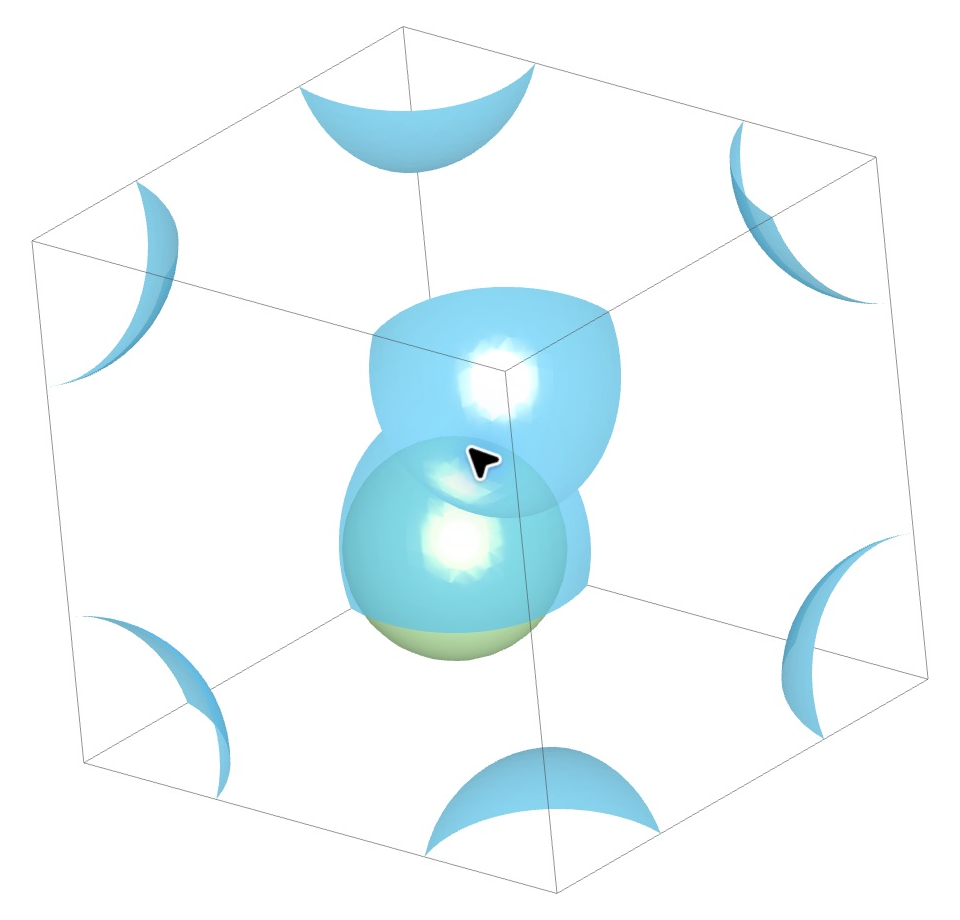
\includegraphics[width=112mm]{publication-assets/crop-53085697480f4dfda16f.png}
\caption{Total charge density from \file{CHGCAR.nospin.gz}. The grid is $32\times32\times32$ and the channel is \ui{Total charge density}. The positive threshold is $0.04000\,\text{\AA}^{-3}$, the negative surface is disabled, and opacity is 0.72.}
\label{fig:volume-total-isosurface}
\end{figure}

\section{Isosurfaces: shapes at a fixed value}
\index{Isosurfaces}

\subsection{What the threshold controls}

An isosurface connects positions with the same scalar value. Raising a positive threshold generally focuses the display on higher-valued regions; lowering it can enlarge or connect surfaces. If no surface appears, first check whether the threshold lies within the data range and whether the channel contains values of the requested sign.

For a scalar field $s(\mathbf r)$ and threshold $\tau$, the isosurface is
\begin{equation}
  S_{\tau}=\{\,\mathbf r\mid s(\mathbf r)=\tau\,\}.
  \label{eq:volume-isosurface}
\end{equation}
The value is fixed, while the data determines the surface's position and shape. A slice instead fixes a spatial plane and colors it according to the values of $s$ on that plane. The two views answer different questions, as illustrated in Figure~\ref{fig:volume-surface-slice-concept}. Direct volume rendering additionally combines information through a volume along each line of sight.

\begin{figure}[htbp]
\centering
\begin{tikzpicture}[x=1mm,y=1mm,font=\sffamily\small]
  \node[text=brand] at (25,45) {Isosurface: fixed value};
  \node[text=brand] at (89,45) {Slice: fixed plane};
  \foreach \dx in {0,64} {
    \draw[draw=muted!55,line width=.4pt]
      ({5+\dx},4) rectangle ({39+\dx},30);
    \draw[draw=muted!55,line width=.4pt]
      ({5+\dx},30) -- ({14+\dx},38) -- ({48+\dx},38)
      -- ({48+\dx},12) -- ({39+\dx},4);
    \draw[draw=muted!55,line width=.4pt] ({39+\dx},30) -- ({48+\dx},38);
    \draw[dashed,draw=muted!40,line width=.4pt]
      ({5+\dx},4) -- ({14+\dx},12) -- ({48+\dx},12);
    \draw[dashed,draw=muted!40,line width=.4pt]
      ({14+\dx},12) -- ({14+\dx},38);
  }
  \filldraw[fill=teal!25,draw=teal,line width=.7pt]
    (26,21) ellipse (13 and 10);
  \draw[draw=teal!65,dashed,line width=.5pt] (13,21) arc (180:0:13 and 3.2);
  \draw[draw=teal!65,line width=.5pt] (13,21) arc (180:360:13 and 3.2);
  \node[text=brand] at (26,25) {$s=\tau$};
  \filldraw[fill=paleblue,draw=brand,line width=.7pt]
    (69,17) -- (103,8) -- (112,25) -- (78,34) -- cycle;
  \begin{scope}
    \clip (69,17) -- (103,8) -- (112,25) -- (78,34) -- cycle;
    \fill[teal!25] (88,21) ellipse (14 and 11);
    \fill[teal!50] (88,21) ellipse (9 and 7);
    \fill[brand!65] (88,21) ellipse (4 and 3.2);
  \end{scope}
  \draw[draw=brand,line width=.7pt]
    (69,17) -- (103,8) -- (112,25) -- (78,34) -- cycle;
  \node[text=ink] at (25,-4) {Shape follows field and threshold};
  \node[text=ink] at (89,-4) {Colors show values on the plane};
\end{tikzpicture}
\caption{Two views of a scalar field (conceptual schematic). An isosurface connects equal values; a slice colors one plane by its field values. Geometry and colors are illustrative.}
\label{fig:volume-surface-slice-concept}
\end{figure}


Select \ui{Isosurfaces} under \ui{Display mode}. Positive and negative surfaces have separate switches and thresholds. Total charge density usually calls for the positive surface; signed fields such as magnetization differences or orbitals may need both. Opacity changes visibility without changing the threshold or source data.

\ui{Isovalue units} offers three threshold conventions: absolute values, standard deviations, and percentiles. Absolute values suit explicit physical thresholds. Standard deviations locate a value relative to the mean and distribution width; percentiles select a position in the value distribution. Use consistent units and record each threshold when comparing absolute distributions between models.

\ui{Absolute value} means entering $\tau$ directly in the selected display units; it does not turn negative values positive. With \ui{Standard deviations (σ)}, the input is a dimensionless multiple $z$ relative to the mean, giving
\begin{equation}
  \tau=\mu+z\sigma.
  \label{eq:volume-sigma-threshold}
\end{equation}
Here $\mu$ and $\sigma$ are the mean and standard deviation of the current channel's grid values. Thus $z=0$ selects the mean and $z=1$ selects one standard deviation above it, rather than a field value of 1. If the mean is nonzero, the threshold cannot be shortened to $z\sigma$.

\begin{table}[htbp]
\centering
\caption{Quantities used for thresholds and color ranges.}
\begin{tabularx}{\linewidth}{lX}
\toprule
Quantity & Meaning in the interface\\
\midrule
$s$, $\tau$ & Current channel value and isosurface threshold; absolute input uses the channel's display units\\
$\mu$, $\sigma$ & Channel mean and standard deviation, in the same units as the values\\
$z$ & Dimensionless number of standard deviations, used to convert a statistical position to a threshold\\
Color limits & The numerical interval covered by the colormap; these do not rewrite field values or CSV data\\
\bottomrule
\end{tabularx}
\end{table}

\ui{Percentile} selects a threshold by ranking the grid samples by value. The 90th percentile, for example, identifies a position in that distribution; it does not mean that the surface encloses 90\% of the electrons or cell volume. Changing channels changes the mean, standard deviation, and percentiles. Record the threshold convention as well as its value when comparing figures.

\subsection{Example: total charge density}

\begin{steps}
  \item Open \file{CHGCAR.nospin.gz}. In the summary, check \ui{Grid} $32\times32\times32$, \ui{Channel} \ui{Total charge density}, and units $\text{\AA}^{-3}$.
  \item Select \ui{Isosurfaces} and set \ui{Isovalue units} to \ui{Absolute value}. Enable \ui{Positive} and enter \literalinput{0.04000} in its \ui{Threshold} field.
  \item Disable \ui{Negative} and set \ui{Opacity} to \literalinput{0.72}. This keeps the surface outline visible while allowing some interior atoms to show through.
  \item Retain \ui{Atoms} and the cell. Temporarily disable \ui{Bonds}, \ui{Depth Cueing}, \ui{Boundary image atoms}, and \ui{One-hop bonded atoms} to focus on the field.
  \item Rotate the view and compare surfaces near the center and boundaries. Record the file, channel, units, threshold, and opacity before exporting a figure.
\end{steps}

Figure~\ref{fig:volume-total-settings} enlarges the summary and settings separately. Use the left panel to identify the dataset and the right panel to identify its display conditions. Grid size, density threshold, and opacity are different kinds of parameters. The value 0.04000 applies to this example; inspect the range before choosing a threshold for another file.

\begin{figure}[H]
\centering
\begin{minipage}[t]{50mm}
\vspace{0pt}
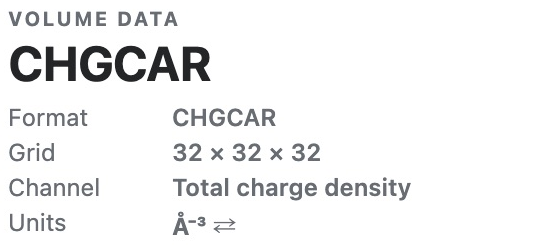
\includegraphics[width=\linewidth]{publication-assets/crop-817224ae41bbaff8bca4.png}
\end{minipage}\hfill
\begin{minipage}[t]{70mm}
\vspace{0pt}
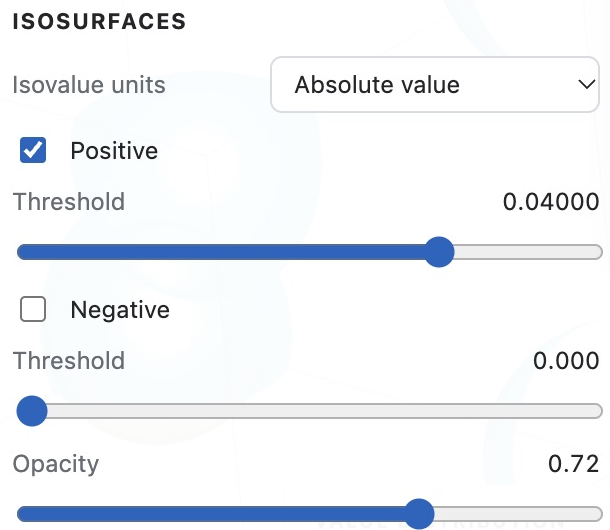
\includegraphics[width=\linewidth]{publication-assets/crop-f580c4c4a5007b46634f.png}
\end{minipage}
\caption{Summary and threshold settings for the same total-density view. The summary lists the grid, channel, and units. The settings use an absolute threshold of 0.04000, no negative surface, and opacity 0.72.}
\label{fig:volume-total-settings}
\end{figure}

\subsection{Example: compare spin channels}

Open \file{CHGCAR.spin.gz}, inspect the total density, then switch to \ui{Magnetization density}, the \file{diff} channel. The summary now shows a $48\times48\times48$ grid. The channel's distribution ranges approximately from $-0.001142$ to $-0.0001356\,\text{\AA}^{-3}$, entirely below zero.

\begin{steps}
  \item Select \ui{Magnetization density}, \ui{Isosurfaces}, and \ui{Absolute value}. Check the channel and units in the summary.
  \item Enable \ui{Negative} and enter \literalinput{-0.0006000} in its \ui{Threshold} field. This lies within the example's range and should produce a red negative isosurface.
  \item Set \ui{Opacity} to \literalinput{0.72}. Keep atoms and the cell, and retain the previous settings that hide bonds and surrounding images. Rotate the view to inspect surfaces inside the cell and near its boundaries.
  \item You can leave \ui{Positive} enabled at threshold 0, as in Figure~\ref{fig:volume-diff-settings}. This file contains no zero or positive values, so that switch adds no positive surface. The green spheres are the atom overlay, controlled separately from surface signs.
  \item Switch to \file{up} and \file{down} to inspect the channels derived from total and difference density. Recheck the range and threshold after each change and record the settings for each channel separately.
\end{steps}

Negative magnetization density means that the difference is negative under the current spin convention, not that total charge density is negative. This example illustrates how the negative-surface switch and threshold work. Showing both signs requires a dataset with the corresponding value range.

\begin{figure}[H]
\centering
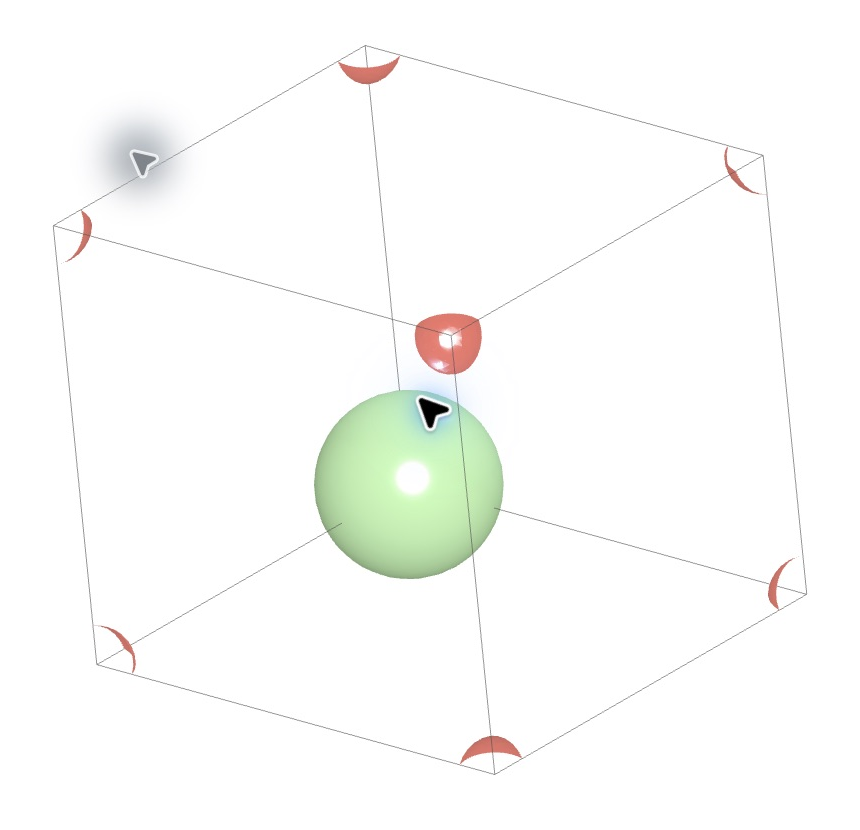
\includegraphics[width=112mm]{publication-assets/crop-eb58a23d11fe997c90a4.png}
\caption{The \ui{Magnetization density} channel in \file{CHGCAR.spin.gz}. The grid is $48\times48\times48$; the red surface has threshold $-0.0006000\,\text{\AA}^{-3}$ and opacity 0.72. Green spheres are the overlaid atoms.}
\label{fig:volume-diff-isosurface}
\end{figure}

\begin{figure}[H]
\centering
\begin{minipage}[t]{50mm}
\vspace{0pt}
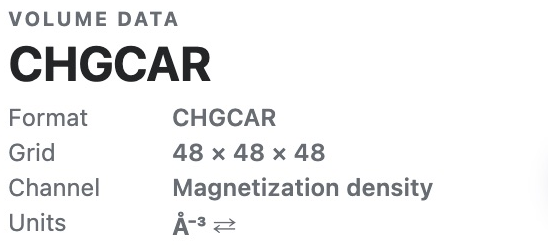
\includegraphics[width=\linewidth]{publication-assets/crop-1252e2f6c064962fc6d9.png}
\end{minipage}\hfill
\begin{minipage}[t]{70mm}
\vspace{0pt}
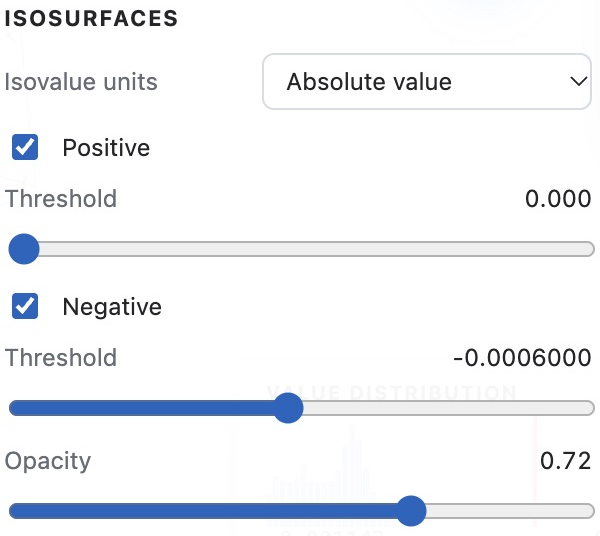
\includegraphics[width=\linewidth]{publication-assets/crop-6e54a4267b5bd8c4b3c0.png}
\end{minipage}
\caption{Magnetization-density summary and thresholds. The positive surface remains enabled at 0 and the negative threshold is $-0.0006000\,\text{\AA}^{-3}$. Since every value is negative, only the negative surface appears.}
\label{fig:volume-diff-settings}
\end{figure}

\subsection{Smoothing and periodic boundaries}

\ui{Smooth vertex normals} improves isosurface lighting by making shading more continuous between triangles. It does not increase the source grid resolution. For periodically sampled data, \ui{Wrap periodic boundaries} connects surfaces across cell boundaries. Enable it only when appropriate to the file's periodicity.

If a surface appears cut off at a boundary, check the cell limits and periodic settings before attributing it to the grid. A higher-quality export sharpens text and edges but cannot compensate for coarse source sampling.

\section{\headinglatin{Miller} slices: inspect internal values}
\index{Slices}
\index{Miller plane slices}

\subsection{One index triplet defines one plane}

Isosurfaces emphasize shapes; slices show continuous variation across a section. After selecting \ui{Miller plane slice}, I, J, and K form one Miller-index triplet defining a single plane through the center of the volumetric data. They cannot all be zero.

For example, $(0,0,1)$ and $(1,0,0)$ select different orientations, while $(1,1,0)$ gives an oblique section. These parameters orient one plane, rather than three independently movable slices. In a nonorthogonal grid, the actual voxel vectors determine the plane's spatial orientation. Do not interpret I, J, and K as Cartesian $x$, $y$, and $z$ sliders.

For a three-dimensional grid with multiple samples in every direction, let $u,v,w$ be normalized positions from the first to last sample along each grid direction, ranging from 0 to 1. Writing the interface's I, J, and K as $h,k,l$, the central plane satisfies
\begin{equation}
  h\left(u-\frac12\right)
  +k\left(v-\frac12\right)
  +l\left(w-\frac12\right)=0.
  \label{eq:volume-central-miller}
\end{equation}
Thus $(0,0,1)$ gives $w=1/2$, and $(1,1,0)$ gives $u+v=1$; both pass through the grid center. These normalized positions span the sampled range and are not universally equivalent to fractional coordinates of a complete cell. The viewer maps the plane into real space using the voxel vectors, preserving the orientation of a skewed grid. Changing the integer triplet rotates the central plane rather than translating it along an axis.

\subsection{Example: the (110) slice of a \headinglatin{Cube} file}

\begin{steps}
  \item Open \file{elec.cube.gz}. Check grid $23\times23\times24$, channel \ui{Dataset 1}, and units \file{arbitrary} in the summary.
  \item Select \ui{Miller plane slice} and set I, J, and K to 1, 1, and 0.
  \item Choose \ui{Cool--warm} under \ui{Colormap} and \ui{Linear} under \ui{Interpolation}. Leave \ui{Range minimum} at \literalinput{0.0034185} and change \ui{Range maximum} to \literalinput{0.2}.
  \item Retain atoms and the cell, set \ui{Atom scale} to \literalinput{0.22}, and hide bonds, coordination polyhedra, depth cueing, and surrounding images so that the tilted plane is clear.
  \item Close the settings panel and rotate the model to inspect where the plane crosses the cell and how atoms lie relative to it. To compare sampling, switch to \ui{Nearest} to see discrete blocks, then return to \ui{Linear}.
  \item Record the indices, colormap, color range, and interpolation, then export PNG or CSV through \ui{Slice export}. The export section below explains their contents.
\end{steps}

Figure~\ref{fig:volume-miller110} uses a relatively low upper color limit to emphasize variation in lower-valued regions. Values above 0.2 use the colormap's high-end color but remain unchanged in the source data and CSV. Red and blue denote the ends of the selected range; color alone does not establish a value's sign.

\begin{figure}[H]
\centering
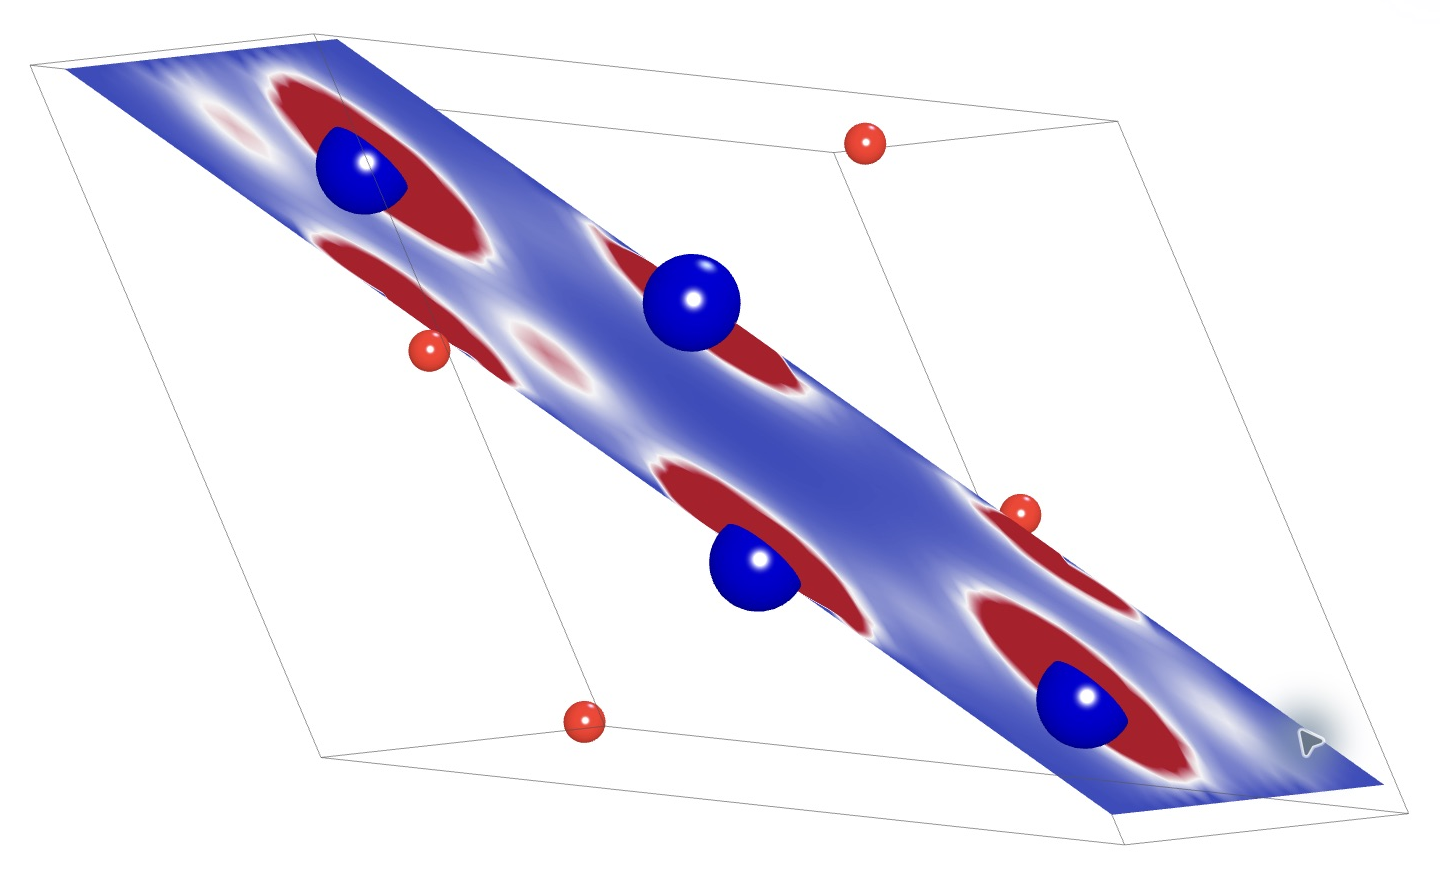
\includegraphics[width=112mm]{publication-assets/crop-aa00ad998951381ace74.png}
\caption{The (110) slice of \file{elec.cube.gz}. Grid $23\times23\times24$, channel \ui{Dataset 1}, units \file{arbitrary}; \ui{Cool--warm}, linear interpolation, and a color range of 0.0034185 to 0.2.}
\label{fig:volume-miller110}
\end{figure}

\begin{figure}[H]
\centering
\begin{minipage}[t]{50mm}
\vspace{0pt}
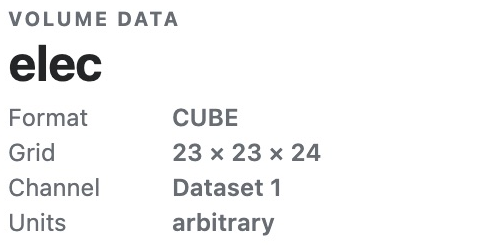
\includegraphics[width=\linewidth]{publication-assets/crop-ab9df592529bd047787b.png}
\end{minipage}\hfill
\begin{minipage}[t]{70mm}
\vspace{0pt}
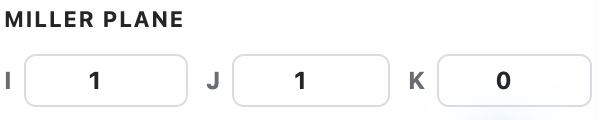
\includegraphics[width=\linewidth]{publication-assets/crop-1de9d3c6e62d7816cea2.png}
\par\vspace{2mm}
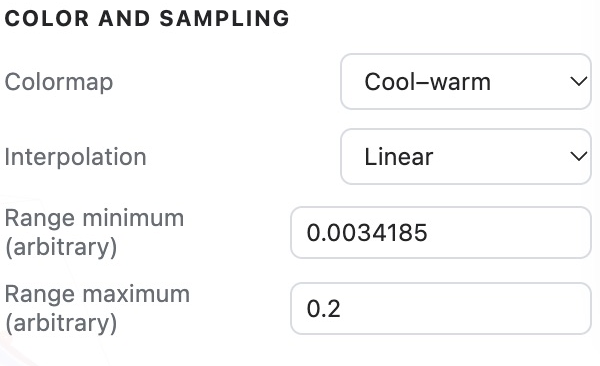
\includegraphics[width=\linewidth]{publication-assets/crop-209a06fc6024f4d5e0ba.png}
\end{minipage}
\caption{Slice summary and settings. The left panel identifies the file, grid, and units. On the right, the upper panel specifies one Miller-index triplet and the lower panel sets colors, interpolation, and range. The upper color limit of 0.2 affects display only.}
\label{fig:volume-miller110-settings}
\end{figure}

You can repeat the exercise with \file{datagrid_3d.xsf}, identifying channels by their labels first. Compare both the grid orientation and the meaning of its scalar values. The same (110) indices do not imply that two files have identical dimensions or numerical ranges.

\subsection{Color ranges and the distribution plot}

\ui{Range minimum} and \ui{Range maximum} map numerical values to the ends of the colormap. A wide range can hide local variation; a narrower one can emphasize the interval of interest. Out-of-range values still exist but use the endpoint colors.

\ui{Value Distribution} shows the current channel's value distribution. In isosurface mode, clicking it sets the corresponding positive or negative threshold. In slice or direct-volume mode, clicking adjusts the nearer color limit; drag the markers for finer adjustment. This is a display-range tool, not an energy spectrum or a profile along a spatial path.

\ui{Cool--warm} often helps distinguish the two signs of a signed field. A sequential colormap is generally easier to read for nonnegative data. Use consistent colormaps and ranges when comparing models, so that color differences have the same meaning.

\section{Direct volume rendering and structure overlays}
\index{Direct volume rendering}

Direct volume rendering accumulates scalar-field colors and opacity along each viewing ray, revealing variation through a volume. Choose \ui{Direct volume (GPU)} under \ui{Display mode}, then adjust opacity, gradient opacity, and sampling quality. \ui{Fast} suits interactive exploration, \ui{Balanced} suits general viewing, and \ui{High} reveals finer detail when the device supports it.

Clipping limits along I, J, and K are fractions from 0 to 1. They hide part of the box to expose the interior. Reducing one direction from 0--1 to 0.25--0.75, for example, isolates its middle region. Clipping changes the displayed extent without deleting data.

\subsection{Example: inspect the central volume along a grid direction}

Continue with \file{elec.cube.gz} to compare slices and volume rendering of the same data. A slice displays values on one plane; volume rendering combines color and opacity along the line of sight. Their brightness need not match point by point.

\begin{steps}
  \item Confirm \file{elec.cube.gz}, \ui{Dataset 1}, grid $23\times23\times24$, and units \file{arbitrary}. Change \ui{Display mode} to \ui{Direct volume (GPU)}.
  \item Retain \ui{Cool--warm}, \ui{Linear}, and the range 0.0034185 to 0.2. Keep colors consistent before comparing the modes.
  \item Set \ui{Sampling quality} to \ui{Balanced}, \ui{Opacity} to \literalinput{0.72}, and \ui{Gradient opacity} to \literalinput{0.35}. Gradient opacity controls how local variation contributes to transparency and can be adjusted separately from overall opacity.
  \item Set the lower and upper \ui{I clipping} limits to \literalinput{0.25} and \literalinput{0.75}. Leave \ui{J clipping} and \ui{K clipping} at 0 and 1. Only the middle half along I is shown; the other directions remain complete.
  \item Retain atoms and the cell; hide bonds, polyhedra, and surrounding images. Close settings and press I to hide the summary and distribution plot. Rotate to inspect continuous internal variation, and press I again whenever you need to check the file information.
\end{steps}

Figure~\ref{fig:volume-direct} shows the result; Figure~\ref{fig:volume-direct-settings} shows the settings. Here I, J, and K specify clipping fractions along grid directions. This differs from the integer triplet defining a Miller slice and need not align with global Cartesian axes. Restore each clipping interval to 0--1 to display the whole volume. The source grid remains $23\times23\times24$.

\begin{figure}[H]
\centering
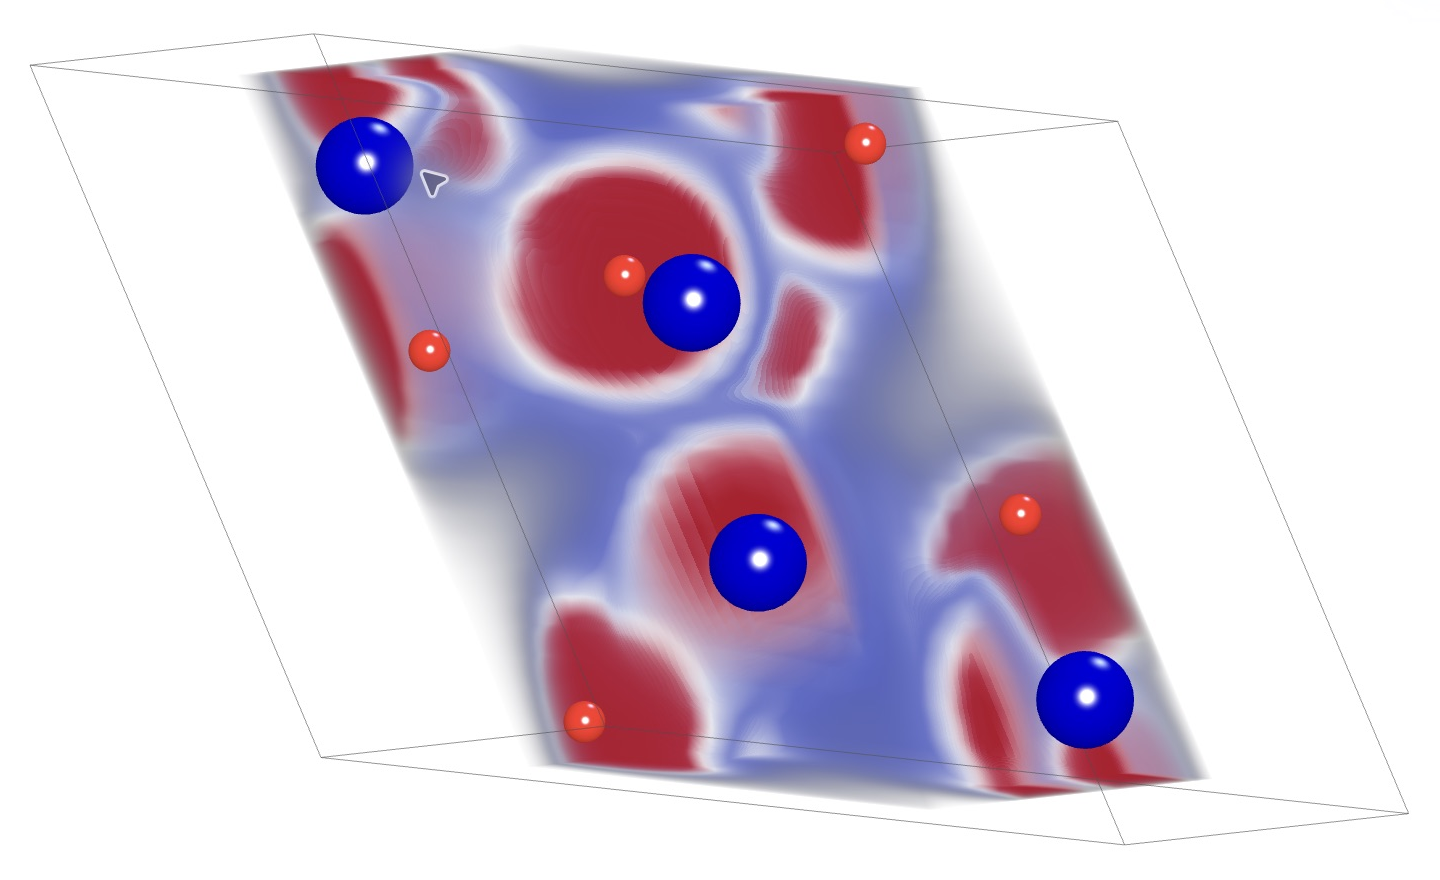
\includegraphics[width=112mm]{publication-assets/crop-68bb0517e51ea1057170.png}
\caption{Direct rendering of \file{elec.cube.gz} using \ui{Direct volume (GPU)}. The \ui{Dataset 1} color range is 0.0034185 to 0.2 and I spans 0.25 to 0.75. Atoms and the full cell outline provide spatial references.}
\label{fig:volume-direct}
\end{figure}

\begin{figure}[H]
\centering
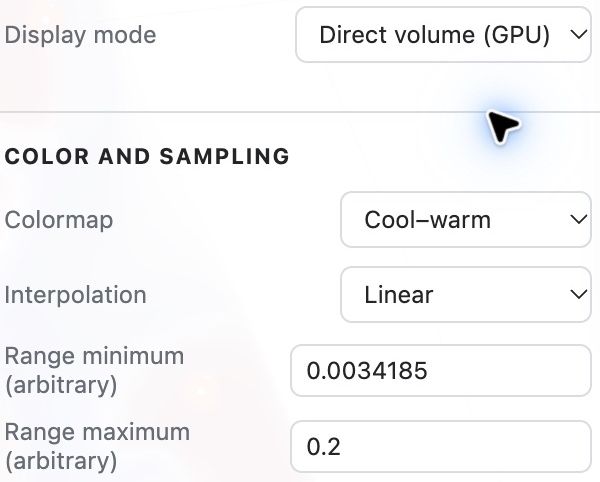
\includegraphics[width=80mm]{publication-assets/crop-3b2d9027085c84d05818.png}
\par\vspace{2mm}
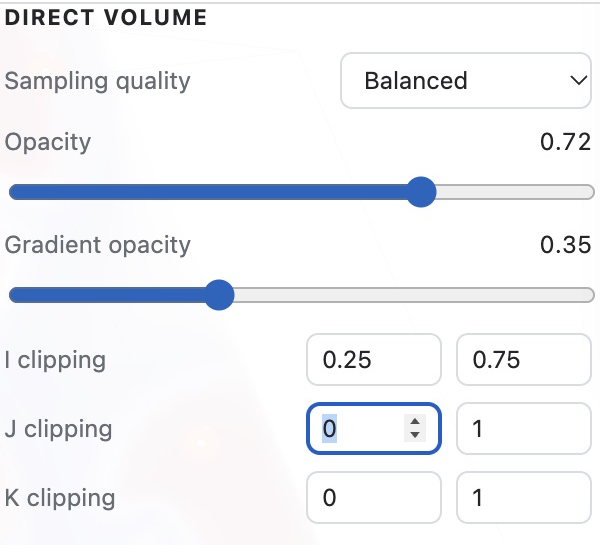
\includegraphics[width=80mm]{publication-assets/crop-7567d94dfd7d877833b9.png}
\caption{Direct-volume settings. Above: mode, colormap, interpolation, and color range. Below: \ui{Balanced} sampling, opacity 0.72, gradient opacity 0.35, and clipping fractions along all three directions.}
\label{fig:volume-direct-settings}
\end{figure}

\subsection{Locate the field using structure overlays}

When the file includes an atomic structure, \ui{Visibility} controls atoms, bonds, the cell, coordination polyhedra, axes, periodic image atoms, magnetic moments, and other objects. Begin with a few useful spatial references, then add overlays individually to keep the field clear.

\ui{Lighting \& surface} controls ambient and directional light, metalness, roughness, brightness, and contrast for the atom overlay. These affect appearance, not the scalar values. Keep them consistent across comparison figures, and state the scientifically meaningful channel, threshold, and units in each caption.

\section{Export volumetric results}
\index{Exporting!Images and data}

\subsection{Sample values in the view}
\index{Sampling values}

Double-click the volume to display a sample value and grid position. The point probe uses trilinear interpolation, so its value need not equal an original grid sample. For precise comparisons, record the channel and sampling position and use the numerical value. Nearest-neighbor and linear slice options govern slice display and export separately; they do not change point-probe interpolation.

Selecting an overlaid atom shows its Cartesian and fractional coordinates in the volume view's atom-information area. Copy buttons retain more precision than the shortened panel display. Atomic coordinates locate an atom; scalar sampling reads the field at a position. These are different kinds of information.

For convertible density units, \ui{Density units} switches between $\text{\AA}^{-3}$ and $\mathrm{bohr}^{-3}$. The displayed number changes while the physical density remains the same. Convert to common units before comparing figures or tabulated values.

\subsection{Export the current image}

The image export menu offers PNG, JPEG, TIFF, SVG, and vector and raster PDF. PNG and TIFF preserve clear raster images; JPEG provides compact files for sharing; SVG and PDF suit document preparation. Stop automatic rotation, choose the view, and check the atoms, cell, and overlays before exporting.

In the text or caption, record the file source, channel, threshold or color range, units, and relevant orientation. Retain the source data as well.

\subsection{Export isosurfaces and slices}
\index{CSV export}

In isosurface mode, \ui{Isosurface export} offers glTF, GLB, PLY, and STL for transferring surface geometry to other 3D tools. The formats preserve different information. Check dimensions and appearance after import elsewhere; coordinates are in \AA.

In slice mode, \ui{Slice export} offers PNG and CSV. PNG saves the colored plane; CSV supports further plotting or numerical analysis. The CSV begins with grid positions \file{i}, \file{j}, and \file{k}, followed by Cartesian positions in \AA: \mbox{\file{x_angstrom}}, \mbox{\file{y_angstrom}}, and \mbox{\file{z_angstrom}}. The final \file{value} column contains source values for the current channel. Samples outside the volume boundary may be invalid; restrict analysis to the valid range.

Reopen the PNG to check orientation, colors, and the region of interest, then inspect the CSV header for coordinate units and the value column. Before plotting matching slices from two models together, ensure that the spatial plane, grid extent, and channel agree. Identical Miller indices specify the same type of direction, but changing the cell can change the plane's real-space size and position.

The example exports \file{elec.total.slice-1_1_0.csv} and a PNG with the same base name. The CSV contains 1568 sampling positions: 778 have finite values and 790 lie outside the volume boundary, with \file{value} recorded as \file{NaN}. NaN is not zero; filter valid values before plotting or calculating statistics.

The finite slice values range approximately from 0.003525 to 2.3995, and 147 exceed the display limit of 0.2. They illustrate the distinction between color settings and source values. The slice PNG is $384\times768$ pixels and shows the plane's color distribution; Figure~\ref{fig:volume-miller110} additionally shows its orientation inside the cell.

\Needspace{8\baselineskip}
\begin{notebox}{Display units and CSV units}
CSV coordinates are exported in \AA, while the value column retains the channel's internal units. For \mbox{CHGCAR}, density values are in $\text{\AA}^{-3}$ even when the interface displays $\mathrm{bohr}^{-3}$. Record Cube and XSF scalar units according to the source file documentation.
\end{notebox}

\ui{Export scene JSON} saves a scene description, including information about the grid, channel, and structure. It does not include the complete voxel array and cannot replace the original field file. Record the camera position and temporary display settings separately. To reproduce an image, retain the source data and note its threshold, color range, and framing.

\subsection{Organize comparable results}

Give matching names to data and figures, including the system, channel, and slice where useful. Keep separate images for CHGCAR \file{total} and \file{diff}; calling both simply a density plot obscures their different meanings. State positive- and negative-surface colors and thresholds in captions, or the color range for slices. Readers should be able to interpret surfaces and colors without opening the original file.

For a research report, keep a working screenshot showing the full summary and settings as well as a clean exported figure. The former helps you check the result; the latter suits presentation. Choose the view according to the feature you want to explain: isosurfaces emphasize shape and connectivity, slices show local variation, and volume rendering conveys spatial depth.

\section{If the image is not what you expected}

For an empty isosurface, check the channel, sign switches, and threshold range. For a nearly uniform slice color, check whether the color range is too broad. If atoms obscure the field, reduce their scale or temporarily hide bonds and polyhedra. Press Space to recenter a model lost during rotation.

Direct volume rendering needs appropriate graphics support. Without WebGL2, the viewer can fall back to CPU slices while retaining slice PNG/CSV export. Insufficient 3D texture capacity can also trigger a slice fallback. Read the stated reason to select a mode supported by the current device. Two-dimensional XSF data is displayed as a slice.

Interpolation, smoothing, and larger exported images improve display only. If your research requires finer spatial information, increase the source grid resolution in the calculation and check convergence again. Only then are the visible details supported by additional data.
